%\renewcommand{\theequation}{\theenumi}
%\begin{enumerate}[label=\arabic*.,ref=\thesubsection.\theenumi]
%\numberwithin{equation}{enumi}
%
%
\item Check which of the following are solutions of the equation 
%
\begin{align}
\myvec{1 & -2}\vec{x} &= 4
\end{align}
%
%
\begin{enumerate}[itemsep=2pt]
\begin{multicols}{2}
\item $\myvec{0 \\ 2}$
\item $\myvec{2 \\ 0}$
\item $\myvec{4 \\ 0}$
\item $\myvec{\sqrt{2} \\ 4\sqrt{2}}$
\item $\myvec{1 \\ 1}$
\end{multicols}
\end{enumerate}
%
\item Find the value of $k$, if $\myvec{2\\1}$ is a solution of the equation 
%
%
\begin{align}
\myvec{2 & 3}\vec{x} &= k
\end{align}
%
%
\item Draw the graphs of the following equations
\begin{enumerate}[itemsep=2pt]
%\begin{multicols}{2}
\item $\myvec{1 & 1}\vec{x} = 4$
\item $\myvec{ 1 & -1}\vec{x}  = 2 $
\item $\myvec{ 3 & -1}\vec{x}  = 0$
\item $\myvec{ 2 & 1}\vec{x}  = 3$
\item $\myvec{ 1 & -1}\vec{x}  = 0$
\item $\myvec{ 1& 1}\vec{x}  = 0$
\item $\myvec{ 2& -1}\vec{x}  = 0$
\item $\myvec{ 7& -3}\vec{x}  = 2$
\item $\myvec{ 1& 1}\vec{x}  = 0$
\item $\myvec{ 1& -1}\vec{x}  = -2$
\item $\myvec{ 1& 1}\vec{x}  = 2$
\item $\myvec{ 1& 2}\vec{x}  = 6$
%\end{multicols}
\end{enumerate}
%
\item Give the equations of two lines passing through \myvec{2 \\ 14}. How many more such lines are there, and why?
\item If the point \myvec{3 \\ 4} lies on the graph of the equation $3y = ax + 7$, find the value of $a$
\\
\solution

The given equation can be expressed as
\begin{align}
\implies \myvec{-a & 3}\vec{x} &= 7
\end{align}
%
$\because$ the given point $\vec{P}$=\myvec{3\\4} satisfies the above equation,
\begin{align}
\myvec{-a & 3}\myvec{3\\4} &= 7
\\
\implies -3a +12 &= 7
\\
\implies a &= \frac{5}{3}
\end{align}

Hence,the equation can be written as 
\begin{align}
\myvec{\frac{-5}{3} & 3}\vec{x} &= 7
\end{align}
and is plotted in Fig. \ref{su2021/2/5/fig:line}.	



\begin{figure}[!ht]
\centering
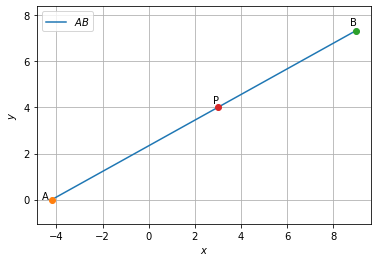
\includegraphics[width=\columnwidth]{solutions/su2021/2/5/Figure4.png}
\caption{Line $AB$}
\label{su2021/2/5/fig:line}	
\end{figure}




\item Find out whether the lines representing the
following pairs of linear equations intersect at a point, are parallel or coincident
%
\begin{enumerate}[itemsep=2pt]
%\begin{multicols}{2}
\item
\begin{align}
\begin{split}
\myvec{5 & -4 }\vec{x}&=-8
\\
\myvec{7 & 6 }\vec{x}&=9
\end{split}
\label{line/6/1.0.1}
\end{align}
\item
\begin{align}
\begin{split}
\myvec{9 & 3 }\vec{x}&=-12
\\
\myvec{18 & 6 }\vec{x}&=-24
\end{split}
\label{line/6/1.0.2}
\end{align}
\item
\begin{align}
\begin{split}
\myvec{6 & -3 }\vec{x}&=-10
\\
\myvec{2 & -1 }\vec{x}&=-9
\end{split}
\label{line/6/1.0.3}
\end{align}
%\end{multicols}
\end{enumerate}
%
\solution
\begin{enumerate}
\item
\begin{align}
\begin{split}
\myvec{5 & -4 }\vec{x}&=-8
\\
\myvec{7 & 6 }\vec{x}&=9
\end{split}
\end{align}
The above equations can be expressed as the matrix equation
\begin{align}
\myvec{5 & -4\\7 & 6} \vec{x} = \myvec{-8\\9}
\end{align}
%
The augmented matrix for the above equation is row reduced as follows
\begin{align}
\myvec{5 & -4 & -8\\7 & 6 & 9} 
\xleftrightarrow {R_1\leftarrow \ 7\frac{R_1}{5}}\myvec{7 & \frac{-28}{5} & \frac{-56}{5}\\7 & 6 & 9} 
\\
%\myvec{7 & \frac{-28}{5} &\frac{-56}{5} \\0 & \frac{58}{5} & \frac{101}{5}} 
\xleftrightarrow {R_2\leftarrow R_2 - R_1}\myvec{7 & \frac{-28}{5} &\frac{-56}{5} \\0 & \frac{58}{5} & \frac{101}{5}}
\\
%\myvec{5 & -4 & -8 \\0 & \frac{58}{5} & \frac{101}{5}} 
\xleftrightarrow {R_1\leftarrow 5\frac{R_1}{7}}\myvec{5 & -4 & -8 \\0 & \frac{58}{5} & \frac{101}{5}}
\\
%\myvec{5 & -4 & -8 \\0 & 58 & 101} 
\xleftrightarrow {R_2\leftarrow 5R_2}\myvec{5 & -4 & -8 \\0 & 58 & 101 }
\end{align}
%
$\because$ row reduction of the $2\times 3$ matrix
%
\begin{align}
\myvec{5 & -4 & -8\\7 & 6 & 9} \label{line/6/2.0.7}
\end{align}
%
results in a matrix with 2 nonzero rows, its rank is 2. 
%
Similarly, the rank of the matrix 
\begin{align}
\myvec{5 & -4 \\7 & 6 } \label{line/6/2.0.8}
\end{align}
%
is also 2.
%
\begin{align}
\because Rank \myvec{5 & -4\\7 & 6} &= Rank\myvec{5 & -4 & -8\\7 & 6 & 9} \nonumber\\
 &=dim \myvec{5 & -4\\7 & 6}\nonumber\\
 &=2
\end{align}

$\therefore$ the lines given in \eqref{line/6/1.0.1} intersect and are plotted in Fig. \ref{line/6/fig:INTERSECTING LINES.}.

\begin{figure}[ht!]
        \centering
        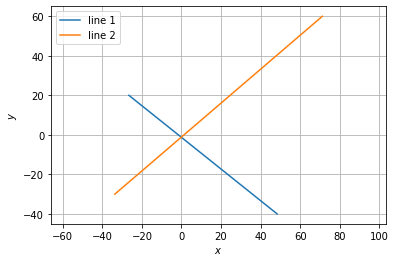
\includegraphics[width=\columnwidth]{solutions/su2021/2/6/FIGURES/INTERSECTING_LINES.png}
        \caption{INTERSECTING LINES.}
        \label{line/6/fig:INTERSECTING LINES.}
    \end{figure} 
    

\item
\begin{align}
\begin{split}
\myvec{9 & 3 }\vec{x}&=-12
\\
\myvec{18 & 6 }\vec{x}&=-24
\end{split}
\end{align}

The above equations can be expressed as the matrix equation
\begin{align}
\myvec{9 & 3\\18 & 6} \vec{x} = \myvec{-12\\-24}
\end{align}
%
The augmented matrix for the above equation is row reduced as follows
\begin{align}
\myvec{9 & 3 & -12\\18 & 6 & -24 } 
\xleftrightarrow {R_1\leftarrow \ 7\frac{R_1}{5}}\myvec{7 & \frac{-28}{5} & \frac{-56}{5}\\7 & 6 & 9} 
\\
%\myvec{18 & 6 & -24} \\18 & 6 & -24 
\xleftrightarrow {R_1\leftarrow \frac{18R_1}{9}}\myvec{18 & 6 & -24 \\18 & 6 & -24}
\\
%\myvec{18 & 6 & -24 \\0 & 0 & 0} 
\xleftrightarrow {R_2\leftarrow R_2-R_1}\myvec{18 & 6 & -24 \\0 & 0 & 0}
\end{align}
%
$\because$ row reduction of the $2\times 3$ matrix
%
\begin{align}
\myvec{9 & 3 & -12\\18 & 6 & -24}
\end{align}
%
results in a matrix with 1 nonzero rows, its rank is 1. 
%
Similarly, the rank of the matrix 
\begin{align}
\myvec{9 & 3 \\18 & 6 } 
\end{align}
%
is also 1.
%
\begin{align}
\because Rank \myvec{9 & 3\\18 & 6} &= Rank\myvec{9 & 3 & -12\\18 & 6 & -24}=1\nonumber\\
&< dim\myvec{9 & 3\\18 & 6}=2
\end{align}
%
$\therefore$ the lines \eqref{line/6/1.0.2} coincide and are plotted in Fig. \ref{line/6/fig:SAME LINES.}.
%
\begin{figure}[ht!]
    \centering
    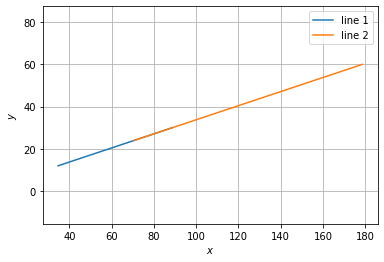
\includegraphics[width=\columnwidth]{solutions/su2021/2/6/FIGURES/SAME_LINES.png}
    \caption{SAME LINES}
    \label{line/6/fig:SAME LINES.}
\end{figure} 
%
\item
\begin{align}
\begin{split}
\myvec{6 & -3 }\vec{x}&=-10
\\
\myvec{2 & -1 }\vec{x}&=-9
\end{split}
\end{align}

The above equations can be expressed as the matrix equation
\begin{align}
\myvec{6 & -3\\2 & -1} \vec{x} = \myvec{-10\\-9}
\end{align}
%
The augmented matrix for the above equation is row reduced as follows
\begin{align}
\myvec{6 & -3 & -10\\2 & -1 & -9 } 
\xleftrightarrow {R_1\leftarrow \ \frac{2R_1}{6}}\myvec{2 & -1 & \frac{-10}{3}\\2 & -1 & -9} 
\\
%\myvec{2 & -1 & \frac{-10}{3} \\0 & 0 & \frac{-17}{3} 
\xleftrightarrow {R_2\leftarrow R_2-R_1}\myvec{2 & -1 & \frac{-10}{3} \\0 & 0 & \frac{-17}{3} }
\\
%\myvec{6 & -3 & -10 \\0 & 0 & \frac{-17}{3}} 
\xleftrightarrow {R_1\leftarrow 3R_1}\myvec{6 & -3 & -10 \\0 & 0 & \frac{-17}{3}} 
\end{align}
%
$\because$ row reduction of the $2\times 3$ matrix
%
\begin{align}
\myvec{6 & -3 & -10\\2 & -1 & -9}
\end{align}
%
results in a matrix with 2 nonzero rows, its rank is 2. 
%
Similarly, the rank of the matrix 
\begin{align}
\myvec{6 & -3 \\2 & -1 } 
\end{align}
%
is 1.
%
\begin{align}
\because Rank \myvec{6 & -3 \\2 & -1 } \ne Rank \myvec{6 & -3 & -10\\2 & -1 & -9}
\end{align}
$\therefore$ the lines in  \eqref{line/6/1.0.3} are parallel and plotted in Fig.     \ref{line/6/fig: PARALLEL lines.}.
%
\begin{figure}[ht]
    \centering
   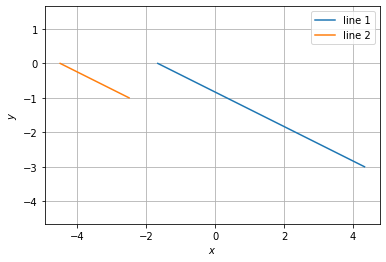
\includegraphics[width=\columnwidth]{solutions/su2021/2/6/FIGURES/PARALLEL_LINES.png}
    \caption{Parallel lines}
    \label{line/6/fig: PARALLEL lines.}
\end{figure}    
\end{enumerate}


\item Find out whether the following pair of linear
equations are consistent, or inconsistent.
%
\begin{enumerate}[itemsep=2pt]
%\begin{multicols}{2}
\item
\begin{align}
\begin{split}
\myvec{3 & 2 }\vec{x}&=5
\\
\myvec{2 & -3 }\vec{x}&=7
\end{split}
\end{align}
\item
\begin{align}
\begin{split}
\myvec{2 & -3 }\vec{x}&=8
\\
\myvec{4 & -6 }\vec{x}&=9
\end{split}
\end{align}
\item
\begin{align}
\begin{split}
\myvec{\frac{3}{2} & \frac{5}{3} }\vec{x}&=7
\\
\myvec{9 & -10 }\vec{x}&=14
\end{split}
\end{align}
\item
\begin{align}
\begin{split}
\myvec{5 & -3 }\vec{x}&=11
\\
\myvec{-10 & 6 }\vec{x}&=-22
\end{split}
\end{align}
\item
\begin{align}
\begin{split}
\myvec{\frac{4}{3} & 2 }\vec{x}&=8
\\
\myvec{2 & 3 }\vec{x}&=12
\end{split}
\end{align}
%\end{multicols}
\end{enumerate}
%
\item Which of the following pairs of linear equations are consistent/inconsistent? If consistent, obtain the solution:
%
\begin{enumerate}[itemsep=2pt]
%\begin{multicols}{2}
\item
\begin{align}
\begin{split}
\myvec{1 & 1 }\vec{x}&=5
\\
\myvec{2 & 2 }\vec{x}&=10
\end{split}
\label{linform/2/8/1.0.1}
\end{align}
\item
\begin{align}
\begin{split}
\myvec{1 & -1 }\vec{x}&=8
\\
\myvec{3 & -3 }\vec{x}&=16
\end{split}
\label{linform/2/8/1.0.2}
\end{align}
\item
\begin{align}
\begin{split}
\myvec{2 & 1 }\vec{x}&=6
\\
\myvec{4 & -2 }\vec{x}&=4
\end{split}
\label{linform/2/8/2/1.0.1}
\end{align}
\item
\begin{align}
\begin{split}
\myvec{2 & -2 }\vec{x}&=2
\\
\myvec{4 & -4 }\vec{x}&=5
\end{split}
\label{linform/2/8/2/1.0.2}
\end{align}
%\end{multicols}
\end{enumerate}
%
\solution
We obtain the vertices of the rhombus as follows
\begin{align}
\vec{A} = \myvec{-3\\0},
\vec{B} = \myvec{0\\-3.5},
\vec{C} = \myvec{3\\0},
\vec{D} = \myvec{0\\3.5}
\end{align}
which are plotted in Fig. \ref{quad/45/fig:Rhombus ABCD}.
%
\begin{figure}[ht!]
\centering
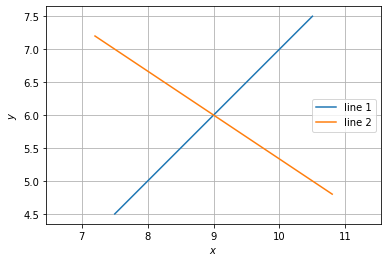
\includegraphics[width=\columnwidth]{solutions/quad/45/figure2.png}
\caption{Rhombus ABCD}
\label{quad/45/fig:Rhombus ABCD}
\end{figure}

We obtain the vertices of the rhombus as follows
\begin{align}
\vec{A} = \myvec{-3\\0},
\vec{B} = \myvec{0\\-3.5},
\vec{C} = \myvec{3\\0},
\vec{D} = \myvec{0\\3.5}
\end{align}
which are plotted in Fig. \ref{quad/45/fig:Rhombus ABCD}.
%
\begin{figure}[ht!]
\centering
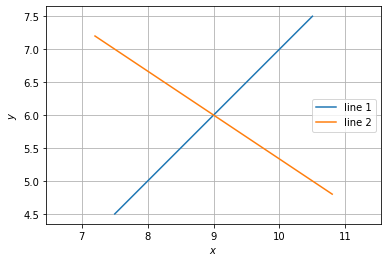
\includegraphics[width=\columnwidth]{solutions/quad/45/figure2.png}
\caption{Rhombus ABCD}
\label{quad/45/fig:Rhombus ABCD}
\end{figure}

\item Given the linear equation $\myvec{2 & 3}\vec{x} – 8 = 0$, write another linear equation in two variables such that the geometrical representation of the pair so formed is: 
%
\begin{enumerate}[itemsep=2pt]
\begin{multicols}{2}
\item  intersecting lines
\item parallel lines 
\item  coincident lines
\end{multicols}
\end{enumerate}
%
\solution
We obtain the vertices of the rhombus as follows
\begin{align}
\vec{A} = \myvec{-3\\0},
\vec{B} = \myvec{0\\-3.5},
\vec{C} = \myvec{3\\0},
\vec{D} = \myvec{0\\3.5}
\end{align}
which are plotted in Fig. \ref{quad/45/fig:Rhombus ABCD}.
%
\begin{figure}[ht!]
\centering
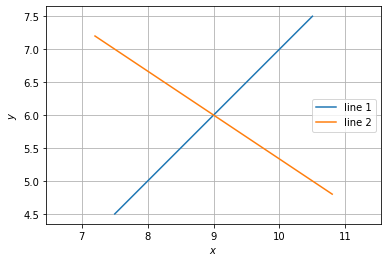
\includegraphics[width=\columnwidth]{solutions/quad/45/figure2.png}
\caption{Rhombus ABCD}
\label{quad/45/fig:Rhombus ABCD}
\end{figure}

%
\item Find the intersection of the following lines
%
\begin{enumerate}[itemsep=2pt]
%\begin{multicols}{2}
\item
\begin{align}
\begin{split}
\myvec{1 & 1 }\vec{x}&=14
\\
\myvec{1 & -1 }\vec{x}&=4
\end{split}
\label{linform/10/ab/1.0.1}
\end{align}
%
%
\item
\begin{align}
\begin{split}
\myvec{1 & -1 }\vec{x}&=3
\\
\myvec{\frac{1}{3} & \frac{1}{2} }\vec{x}&=6
\end{split}
\label{linform/10/ab/1.0.2}
\end{align}
\item
\begin{align}
\begin{split}
\myvec{3 & -1 }\vec{x}&=3
\\
\myvec{9 & -3 }\vec{x}&=9
\end{split}
\label{linform/10/1.0.1}
\end{align}
\item
\begin{align}
\begin{split}
\myvec{0.2 & 0.3 }\vec{x}&=1.3
\\
\myvec{0.4 & 0.5 }\vec{x}&=2.3
\end{split}
\label{linform/10/1.0.2}
\end{align}
\item
\begin{align}
\begin{split}
\myvec{\sqrt{2} & \sqrt{3} }\vec{x}&=0
\\
\myvec{\sqrt{3} & \sqrt{8} }\vec{x}&=0
\end{split}
\end{align}
\item
\begin{align}
\begin{split}
\myvec{\frac{3}{2} & -\frac{5}{3} }\vec{x}&=-2
\\
\myvec{\frac{1}{3} & \frac{1}{2} }\vec{x}&=\frac{13}{6}
\end{split}
\end{align}
%\end{multicols}
\end{enumerate}
%
\solution

We obtain the vertices of the rhombus as follows
\begin{align}
\vec{A} = \myvec{-3\\0},
\vec{B} = \myvec{0\\-3.5},
\vec{C} = \myvec{3\\0},
\vec{D} = \myvec{0\\3.5}
\end{align}
which are plotted in Fig. \ref{quad/45/fig:Rhombus ABCD}.
%
\begin{figure}[ht!]
\centering
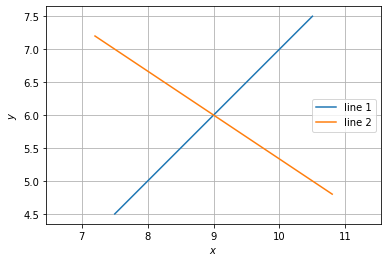
\includegraphics[width=\columnwidth]{solutions/quad/45/figure2.png}
\caption{Rhombus ABCD}
\label{quad/45/fig:Rhombus ABCD}
\end{figure}

%
\item
\begin{align}
\begin{split}
\myvec{3 & -1 }\vec{x}&=3
\\
\myvec{9 & -3}\vec{x}&=9
\end{split}
\end{align}
The above equations can be expressed as the matrix equation
\begin{align}
\myvec{3 & -1\\9 & -3} \vec{x} = \myvec{3\\9}
\end{align}
%
Now we converted these matrix equation in augmented matrix form using row reduction
\begin{align}
\myvec{3 & -1 & 3\\9 & -3 & 9} 
\xleftrightarrow {R_2\rightarrow \ \frac{R_2}{3}}\myvec{3 & -1 & 3\\3 & -1 & 3} 
\end{align}
%
Since the rows are linearly dependent, the given set of equations has infinite solutions and the lines are coincident
as can be seen from Fig. \ref{linform/10/fig:SAME LINES.}.
%
\begin{figure}[ht!]
\centering
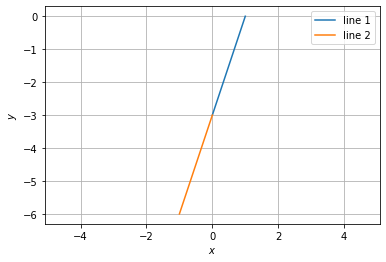
\includegraphics[width=\columnwidth]{solutions/su2021/2/10/FIGURES/SAME-LINE.png}
\caption{SAME-LINES}
\label{linform/10/fig:SAME LINES.}
\end{figure} 
%
\item
\begin{align}
\begin{split}
\myvec{0.2 & 0.3 }\vec{x}&=1.3
\\
\myvec{0.4 & 0.5}\vec{x}&=2.3
\end{split}
\end{align}
The above equations can be expressed as the matrix equation
\begin{align}
\myvec{0.2 & 0.3\\0.4 & 0.5} \vec{x} = \myvec{1.3\\1.4}
\end{align}
%
Now we converted these matrix equation in augmented matrix form using row reduction
\begin{align}
\myvec{0.2 & 0.3 & 1.3\\0.4 & 0.5 & 1.4 } 
\xleftrightarrow {R_2\rightarrow R_2-2R_1}\myvec{0.2 & 0.3 & 1.3\\0 & -0.1 & -0.3} 
\\
%\myvec{0.2 & 0.3 & 1.3} \\0 & 1 & 3
\xleftrightarrow {R_2\rightarrow \frac{R_2}{-0.1}}\myvec{0.2 & 0.3 & 1.3 \\0 & 1 & 3}
\\
%\myvec{0.2 & 0 & 0.4 \\0 & 1 & 3} 
\xleftrightarrow {R_1\rightarrow R_1-0.3R_2}\myvec{0.2 & 0 & 0.4 \\0 & 1 & 3}
\\
%\myvec{1 & 0 & 2\\ 0 & 1 & 3}
\xleftrightarrow {R_1\rightarrow \frac{R_1}{0.2}}\myvec{1 & 0 & 2 \\0 & 1 & 3}
\end{align}
%
Thus, the point of intersection is \myvec{2\\3}, as can be seen from Fig. \ref{linform/10/fig:INTERSECTING LINES.}
%
\begin{figure}[ht!]
\centering
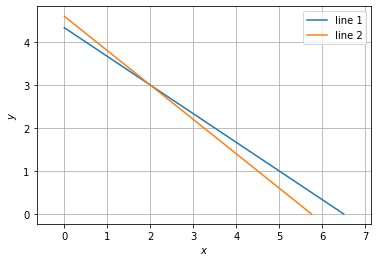
\includegraphics[width=\columnwidth]{solutions/su2021/2/10/FIGURES/INTERSECTING-LINE.png}
\caption{INTERSECTING-LINES}
\label{linform/10/fig:INTERSECTING LINES.}
\end{figure} 
\end{enumerate}


We obtain the vertices of the rhombus as follows
\begin{align}
\vec{A} = \myvec{-3\\0},
\vec{B} = \myvec{0\\-3.5},
\vec{C} = \myvec{3\\0},
\vec{D} = \myvec{0\\3.5}
\end{align}
which are plotted in Fig. \ref{quad/45/fig:Rhombus ABCD}.
%
\begin{figure}[ht!]
\centering
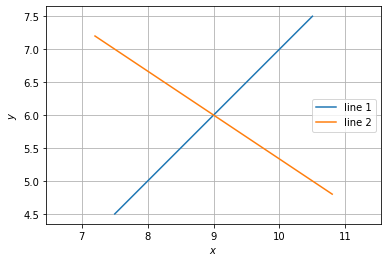
\includegraphics[width=\columnwidth]{solutions/quad/45/figure2.png}
\caption{Rhombus ABCD}
\label{quad/45/fig:Rhombus ABCD}
\end{figure}

%
%
\item Which of the following pairs of linear equations has a unique solution, no solution, or infinitely many solutions?
%
\begin{enumerate}[itemsep=2pt]
%\begin{multicols}{2}
\item
\begin{align}
\begin{split}
\myvec{1 & -3 }\vec{x}&=3
\\
\myvec{3 & -9 }\vec{x}&=2
\end{split}
\label{linform/11/ab/1.0.1}
\end{align}
\item
\begin{align}
\begin{split}
\myvec{2 & 1 }\vec{x}&=5
\\
\myvec{3 & 2 }\vec{x}&=8
\end{split}
\label{linform/11/ab/1.0.2}
\end{align}
\item
\begin{align}
\begin{split}
\myvec{3 & -5 }\vec{x}&=20
\\
\myvec{6 & -10 }\vec{x}&=40
\end{split}
\end{align}
\item
\begin{align}
\begin{split}
\myvec{1 & -3 }\vec{x}&=7
\\
\myvec{3 & -3 }\vec{x}&=15
\end{split}
\end{align}
%\end{multicols}
\end{enumerate}
%
\solution
\begin{enumerate}
We obtain the vertices of the rhombus as follows
\begin{align}
\vec{A} = \myvec{-3\\0},
\vec{B} = \myvec{0\\-3.5},
\vec{C} = \myvec{3\\0},
\vec{D} = \myvec{0\\3.5}
\end{align}
which are plotted in Fig. \ref{quad/45/fig:Rhombus ABCD}.
%
\begin{figure}[ht!]
\centering
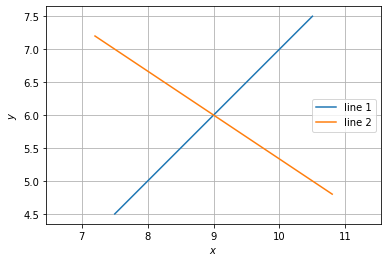
\includegraphics[width=\columnwidth]{solutions/quad/45/figure2.png}
\caption{Rhombus ABCD}
\label{quad/45/fig:Rhombus ABCD}
\end{figure}
    
We obtain the vertices of the rhombus as follows
\begin{align}
\vec{A} = \myvec{-3\\0},
\vec{B} = \myvec{0\\-3.5},
\vec{C} = \myvec{3\\0},
\vec{D} = \myvec{0\\3.5}
\end{align}
which are plotted in Fig. \ref{quad/45/fig:Rhombus ABCD}.
%
\begin{figure}[ht!]
\centering
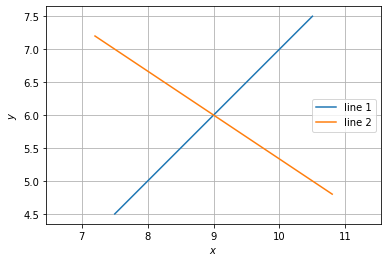
\includegraphics[width=\columnwidth]{solutions/quad/45/figure2.png}
\caption{Rhombus ABCD}
\label{quad/45/fig:Rhombus ABCD}
\end{figure}

\end{enumerate}
%



\item Find the slope of the line, which makes an angle of $30\degree$ of y-axis measured anticlockwise.
\item Write the equations for the x and y axes.
\item Find the equation of the line satisfying the following conditions 
\begin{enumerate}
\item passing through  the point \myvec{-4\\3} with slope $\frac{1}{2}$.
\item passing through the point \myvec{0\\0} with slope $m$.
\item passing through the point $\myvec{2\\2\sqrt{3}}$ and inclined with the x-axis at an angle of 75$\degree$.
\item Intersecting the x-axis at a distance of 3 units to the let of the origin with slope -2.
\item intersecting the y-axis at a distance of 2 units above the origin and making an angle of $30\degree$ with the positive direction of the x-axis.
\item passing through the points \myvec{-1\\1} and \myvec{2\\-4}.
\item perpendicular distance from the origin is 5 and the angle made by the perpendicular with the positive x-axis is 30$\degree$.
\end{enumerate}
%
\solution
\begin{enumerate}
    \item Given point $\vec{P} = \myvec{-4\\3}$ and slope $m = \frac{1}{2}$.
    The direction vector is $\vec{m} = \myvec{2\\1}$.  
    Hence, the normal vector
    \begin{align}
    \label{linform/2/14/eq:line_norm_dir}
    \vec{n} &= \myvec{0&-1\\1&0}\vec{m} 
    \\
    &= \myvec{-1\\2}
    \end{align}
    The equation of the line in terms of the normal vector is then obtained as
    \begin{align}
    \label{linform/2/14/eq:line_norm_vec}
    \vec{n}^T\brak{\vec{x}-\vec{A}} &= 0
    \\
    \implies \myvec{-1 & 2} \vec{x} &= 10
    \end{align}
    See Fig.     \ref{linform/2/14/Plot of Line $AB$ (Part-1)}
    \begin{figure}[ht]
    \centering
    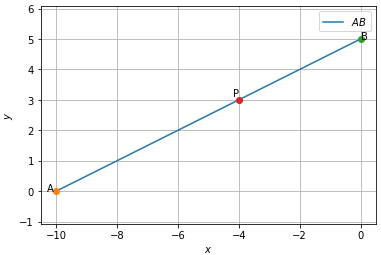
\includegraphics[width=\columnwidth]{solutions/su2021/2/14/Line_Plot_Part1.PNG}
    \caption{Plot of Line $AB$ (Part-1)}
    \label{linform/2/14/Plot of Line $AB$ (Part-1)}
    \end{figure}
    \item Given point $\vec{P} = \myvec{2\\2\sqrt{3}}$.From the given information we have, $\tan75\degree =m = \frac{\sqrt{3}+1}{\sqrt{3}-1}$.
    The direction vector is $\vec{m} = \myvec{1\\\tan75\degree}$.  
    Hence, the normal vector
    \begin{align}
    \label{linform/2/14/eq:line_norm_dir2}
    \vec{n} &= \myvec{0&-1\\1&0}\vec{m} 
    \\
    &= \myvec{-\tan75\degree\\1}
    \end{align}
    The equation of the line in terms of the normal vector is then obtained as
    \begin{align}
    \label{linform/2/14/eq:line_norm_vec2}
    \vec{n}^T\brak{\vec{x}-\vec{A}} &= 0
    \\
    \implies \myvec{-\sqrt{3}+1 &\sqrt{3}-1}  \vec{x} &= -4\brak{\sqrt{3}-1}
    \end{align}
    See Fig. \ref{linform/2/14/Plot of Line $AB$ (Part-2)}

    \begin{figure}[ht]
    \centering
    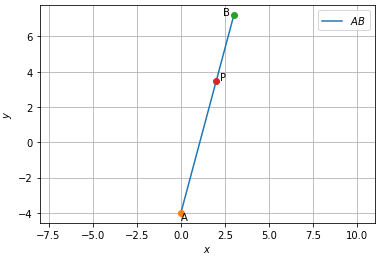
\includegraphics[width=\columnwidth]{solutions/su2021/2/14/Line_Plot_Part2.PNG}
    \caption{Plot of Line $AB$ (Part-2)}
    \label{linform/2/14/Plot of Line $AB$ (Part-2)}
    \end{figure}
\end{enumerate}
We obtain the vertices of the rhombus as follows
\begin{align}
\vec{A} = \myvec{-3\\0},
\vec{B} = \myvec{0\\-3.5},
\vec{C} = \myvec{3\\0},
\vec{D} = \myvec{0\\3.5}
\end{align}
which are plotted in Fig. \ref{quad/45/fig:Rhombus ABCD}.
%
\begin{figure}[ht!]
\centering
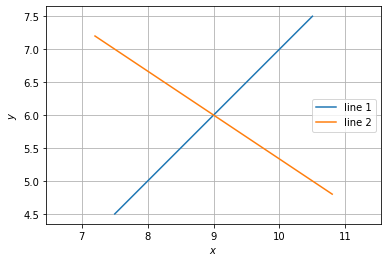
\includegraphics[width=\columnwidth]{solutions/quad/45/figure2.png}
\caption{Rhombus ABCD}
\label{quad/45/fig:Rhombus ABCD}
\end{figure}


\item Find the equation of the line passing through \myvec{-3\\5} and perpendicular to the line through the points \myvec{2\\5} and \myvec{-3\\6}.
%
\solution
We obtain the vertices of the rhombus as follows
\begin{align}
\vec{A} = \myvec{-3\\0},
\vec{B} = \myvec{0\\-3.5},
\vec{C} = \myvec{3\\0},
\vec{D} = \myvec{0\\3.5}
\end{align}
which are plotted in Fig. \ref{quad/45/fig:Rhombus ABCD}.
%
\begin{figure}[ht!]
\centering
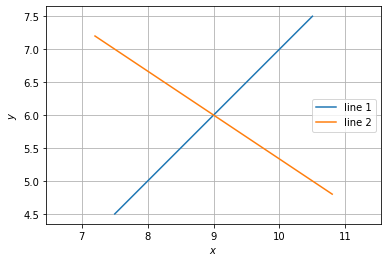
\includegraphics[width=\columnwidth]{solutions/quad/45/figure2.png}
\caption{Rhombus ABCD}
\label{quad/45/fig:Rhombus ABCD}
\end{figure}


\item Find the direction vectors and and y-intercepts  of the following lines 
\begin{enumerate}
\item $\myvec{1 & 7}\vec{x} = 0$.
\item $\myvec{6 & 3}\vec{x} = 5$.
\item $\myvec{0 & 1}\vec{x} = 0$.
\end{enumerate}

\item Find the perpendicular distances of the following lines from the origin and angle between the perpendicular and the positive x-axis.
\begin{enumerate}
\item $\myvec{1 & -\sqrt{3}}\vec{x} = -8$.
\item $\myvec{0 & 1}\vec{x} = 2$.
\item $\myvec{1 & -1}\vec{x} = 4$.
\end{enumerate}
\item Find the distance between the parallel lines
%
\begin{align}
\myvec{15 & 8}\vec{x} &= 34
\\
\myvec{15 & 8}\vec{x} &= -31
\end{align}
%
\solution

    The distance between the two parallel lines is 
    \begin{align}
    d = \frac{\abs{c_2-c_1}}{\norm{\vec{n}}}
    \end{align}
    By substituting the given values 
    \begin{align}
     \vec{n} = \myvec{15 \\ 8}, c_1=34,c_2=-31
    \end{align}
    we get  
    \begin{align}
    d=\frac{{65}}{17}
    \end{align}



\item Find the equation of the line parallel to the line 
\begin{align}
\myvec{3 & -4}\vec{x} = -2
\end{align}
%
and passing through the point \myvec{-2\\3}.
\item Find the alue of $p$ so that the three lines 
%
\begin{align}
\myvec{3 & 1}\vec{x} &= 2
\\
\myvec{p & 2}\vec{x} &= 3
\\
\myvec{2 & -1}\vec{x} &= 3
\end{align}
%
may intersect at one point.
%
\solution
We obtain the vertices of the rhombus as follows
\begin{align}
\vec{A} = \myvec{-3\\0},
\vec{B} = \myvec{0\\-3.5},
\vec{C} = \myvec{3\\0},
\vec{D} = \myvec{0\\3.5}
\end{align}
which are plotted in Fig. \ref{quad/45/fig:Rhombus ABCD}.
%
\begin{figure}[ht!]
\centering
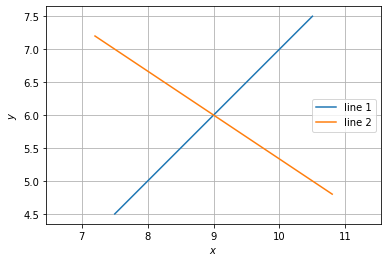
\includegraphics[width=\columnwidth]{solutions/quad/45/figure2.png}
\caption{Rhombus ABCD}
\label{quad/45/fig:Rhombus ABCD}
\end{figure}

%
\item The hypotenuse of a right angled triangle has its ends at the points \myvec{1\\3} and \myvec{-4\\1}. Find an equation of the legs of the triangle.

\item If the lines
%
%
\begin{align}
\myvec{-3 & 1}\vec{x} &= 1
\\
\myvec{-1 & 2}\vec{x} &= 3
\end{align}
%
are equally inclined to the line
%
\begin{align}
\myvec{-m & 1}\vec{x} &= 4,
\end{align}
%
find the value of $m$.
%
\item The sum of the perpendicular distances of a variable point $\vec{P}$ from the lines
%
\begin{align}
\myvec{1 & 1}\vec{x} &= 0
\\
\myvec{3 & -2}\vec{x} &= -7
\end{align}
%
is always 10.  Show that $\vec{P}$ must move on a line.
%
\item Find the equation of the line which is equidistant from parallel lines
%
\begin{align}
\myvec{9 & 7}\vec{x} &= 7
\\
\myvec{3 & 2}\vec{x} &= -6.
\end{align}
%
\item Determine the ratio in which the line 
\begin{align}
\myvec{2 & 1}\vec{x} - 4 = 0
\end{align}
%
divides the line segment joining the points $\vec{A}=\myvec{2\\-2}, \vec{B}=\myvec{3\\7}$.
\item A line perpendicular to the line segment joining the points \myvec{1\\0} and \myvec{2\\3} divides it in the ratio $1:n$.  Find the equation of the line.
\item Find the equation of a line that cuts off equal intercepts on the coordinate axes and passes through the point \myvec{2\\3}.
\item Find the equation of the line passing through the point \myvec{2\\2} and cutting off intercepts on the axes whose sum is 9.
\item Find the equation of the line through the point \myvec{0\\2} making an angle $\frac{2\pi}{3}$ with the positive x-axis.  Also, find the equation of the line parallel to it and crossing the y-axis at a distance of 2 units below the origin.
\item The perpendicular from the origin to a line meets it at a point \myvec{-2\\9}, find the equation of the line.
\item Find the angle between the following pair of lines:
\begin{align}
L_1: \quad \vec{x} &= \myvec{3\\1\\-2} + \lambda_1\myvec{1 \\ -1 \\-2}
\\
L_2: \quad \vec{x} &= \myvec{2\\-1\\-56} + \lambda_2\myvec{3 \\ -5 \\-4}
\end{align}
%\end{enumerate}
\item Find the shortest distance between the lines 
\begin{align}
L_1: \quad \vec{x} &= \myvec{1\\2\\1} + \lambda_1\myvec{1 \\ -1 \\1}
\\
L_2: \quad \vec{x} &= \myvec{2\\-1\\-1} + \lambda_2\myvec{2 \\ 1 \\2}
\end{align}
\solution
We obtain the vertices of the rhombus as follows
\begin{align}
\vec{A} = \myvec{-3\\0},
\vec{B} = \myvec{0\\-3.5},
\vec{C} = \myvec{3\\0},
\vec{D} = \myvec{0\\3.5}
\end{align}
which are plotted in Fig. \ref{quad/45/fig:Rhombus ABCD}.
%
\begin{figure}[ht!]
\centering
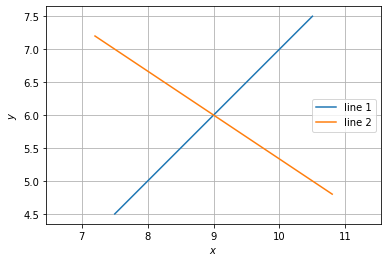
\includegraphics[width=\columnwidth]{solutions/quad/45/figure2.png}
\caption{Rhombus ABCD}
\label{quad/45/fig:Rhombus ABCD}
\end{figure}

%
\item Find the shortest distance between the lines 
\begin{align}
\frac{x+1}{7} = \frac{y+1}{-6} &= \frac{z+1}{1}, 
\\
\frac{x-3}{1} = \frac{y-5}{-2} &= \frac{z-7}{1} 
\end{align}
%
\item Find the shortest distance between the lines 
\begin{align}
L_1: \quad \vec{x} &= \myvec{1\\2\\3} + \lambda_1\myvec{1 \\ -3 \\2}
\\
L_2: \quad \vec{x} &= \myvec{4\\5\\6} + \lambda_2\myvec{2 \\ 3 \\1}
\end{align}
%
\item Find the equation of the planes
\begin{enumerate}
\item that passes through the point \myvec{1\\0\\-2} and the normal to the plane is \myvec{1\\1\\-1}.
\\
\solution
The equation of the plane is given by 
\begin{align}
\vec{n}^T\brak{\vec{x}-\vec{A}} &= 0
\\
\implies \myvec{1 & 1 & -1}{\vec{x}} &= \myvec{1 & 1 & -1}{\myvec{1\\0\\-2}}
\\
\text{or, }\myvec{1 & 1 & -1}{\vec{x}} &= 3
\end{align}
and plotted in Fig. \ref{linform/35/1/Plot of the plane}.

\begin{figure}[ht]
\centering
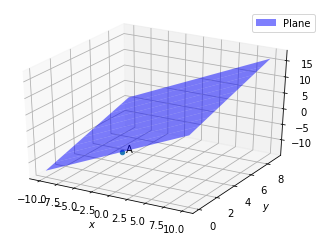
\includegraphics[width=\columnwidth]{solutions/su2021/2/35/1/Plane_plot1.PNG}
\caption{Plot of the plane}
\label{linform/35/1/Plot of the plane}
\end{figure}


\item that passes through the point \myvec{1\\4\\6} and the normal vetor the plane is \myvec{1\\-2\\1}.
\solution
We obtain the vertices of the rhombus as follows
\begin{align}
\vec{A} = \myvec{-3\\0},
\vec{B} = \myvec{0\\-3.5},
\vec{C} = \myvec{3\\0},
\vec{D} = \myvec{0\\3.5}
\end{align}
which are plotted in Fig. \ref{quad/45/fig:Rhombus ABCD}.
%
\begin{figure}[ht!]
\centering
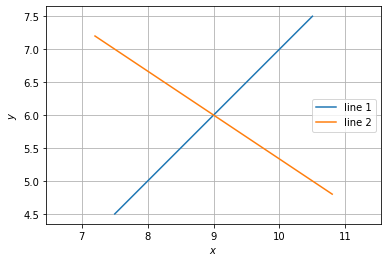
\includegraphics[width=\columnwidth]{solutions/quad/45/figure2.png}
\caption{Rhombus ABCD}
\label{quad/45/fig:Rhombus ABCD}
\end{figure}


\end{enumerate}
\item Find the equation of the planes that passes through three points
\begin{enumerate}
\item \myvec{1\\1\\-1}, \myvec{6\\4\\-5}, \myvec{-4\\-2\\3}
\item \myvec{1\\1\\0}, \myvec{1\\2\\1}, \myvec{-2\\2\\-1}.
\end{enumerate}
\solution
\begin{enumerate}
    \item 

If the equation of the plane is given by
\begin{align}
\vec{n}^T\vec{x} = 1,
\end{align}
\begin{align}
\myvec{1&1&-1 \\ 6&4&-5 \\ -4&-2&3} \vec{n} &= \myvec{1\\1\\1}
\end{align}
Row reducing the augmented matrix, 
\begin{align}
\myvec{1 & 0 & -0.5 & -1.5\\0 & 1 & -0.5 & 2.5\\0 & 0 & 0 & 0}
\end{align}
which yields the  equation of the line
\begin{align}
\vec{x} &= \myvec{1 \\ 6 \\ -4}+\lambda\myvec{0 \\ -2 \\2}
\end{align}
and is plotted in Fig. \ref{linform/38/a/Plot of the line}.
\begin{figure}[ht]
\centering
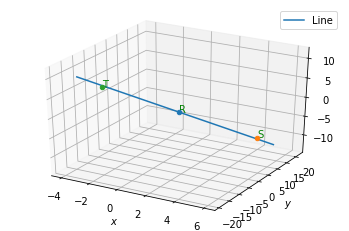
\includegraphics[width=\columnwidth]{solutions/su2021/2/36/a/download (5).png}
\caption{plot of the line}
\label{linform/38/a/Plot of the line}
\end{figure}



\end{enumerate}
\item Find the intercepts cut off by the plane 
$
\myvec{2 & 1 & 1}\vec{x}=5.
$
\item Find the equaion of the plane with intercept 3 on the y-axis and parallel to ZOX plane.
\item Find the equation of the plane through the intersection of the planes 
$
\myvec{3 & -1 & 2}\vec{x}=4
$
 and 
$
\myvec{1 & 1 & 1}\vec{x}=-2
$
and the pont \myvec{2\\2\\1}.
%
\\
\solution
We obtain the vertices of the rhombus as follows
\begin{align}
\vec{A} = \myvec{-3\\0},
\vec{B} = \myvec{0\\-3.5},
\vec{C} = \myvec{3\\0},
\vec{D} = \myvec{0\\3.5}
\end{align}
which are plotted in Fig. \ref{quad/45/fig:Rhombus ABCD}.
%
\begin{figure}[ht!]
\centering
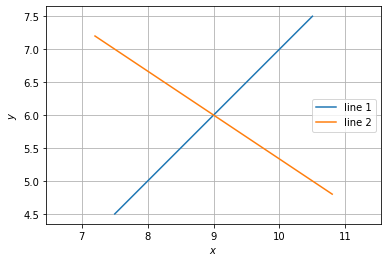
\includegraphics[width=\columnwidth]{solutions/quad/45/figure2.png}
\caption{Rhombus ABCD}
\label{quad/45/fig:Rhombus ABCD}
\end{figure}


\item Find the equation of the plane passing through the intersection of the planes 
$
\myvec{2 & 2 & -3}\vec{x}=7
$
 and 
$
\myvec{2 & 5 & 3}\vec{x}=9
$
and the pont \myvec{2\\1\\3}.
%
\item  Find the equation of the plane through the intersection of the planes
$
\myvec{1 & 1 & 1}\vec{x}=1
$
 and 
$
\myvec{2 & 3 & 4}\vec{x}=5
$
which is perpendicular to the plane 
$
\myvec{1 & -1 & 1}\vec{x}=0.
$
%
\item Find the angle between the planes whose equations are
$
\myvec{2 & 2 & -3}\vec{x}=5
$
 and 
$
\myvec{3 & -3 & 5}\vec{x}=3
$
\\
\solution
We obtain the vertices of the rhombus as follows
\begin{align}
\vec{A} = \myvec{-3\\0},
\vec{B} = \myvec{0\\-3.5},
\vec{C} = \myvec{3\\0},
\vec{D} = \myvec{0\\3.5}
\end{align}
which are plotted in Fig. \ref{quad/45/fig:Rhombus ABCD}.
%
\begin{figure}[ht!]
\centering
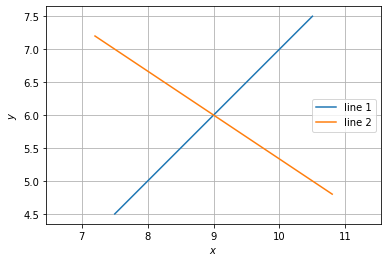
\includegraphics[width=\columnwidth]{solutions/quad/45/figure2.png}
\caption{Rhombus ABCD}
\label{quad/45/fig:Rhombus ABCD}
\end{figure}

%
\item In the following cases, determine whether the given planes are parallel or perpendicular, and in case they are neither, find the angles between them.
\begin{enumerate}
\item 
$
\myvec{7 & 5 & 6}\vec{x}=-30
$
 and 
$
\myvec{3 & -1 & -10}\vec{x}=-4
$
%
\item 
$
\myvec{2 & 1 & 3}\vec{x}=2
$
 and 
$
\myvec{1 & -2 & 5}\vec{x}=0
$
%
\item 
$
\myvec{2 & -2 & 4}\vec{x}=-5
$
 and 
$
\myvec{3 & -3 & 6}\vec{x}=1
$
\item 
$
\myvec{2 & -1 & 3}\vec{x}=1
$
 and 
$
\myvec{2 & -1 & 3}\vec{x}=-3
$
\item 
$
\myvec{4 & 8 & 1}\vec{x}=8
$
 and 
$
\myvec{0 & 1 & 1}\vec{x}=4
$
\end{enumerate}
\solution
\begin{enumerate}
    \item 
    We obtain the vertices of the rhombus as follows
\begin{align}
\vec{A} = \myvec{-3\\0},
\vec{B} = \myvec{0\\-3.5},
\vec{C} = \myvec{3\\0},
\vec{D} = \myvec{0\\3.5}
\end{align}
which are plotted in Fig. \ref{quad/45/fig:Rhombus ABCD}.
%
\begin{figure}[ht!]
\centering
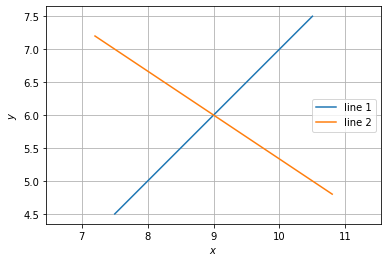
\includegraphics[width=\columnwidth]{solutions/quad/45/figure2.png}
\caption{Rhombus ABCD}
\label{quad/45/fig:Rhombus ABCD}
\end{figure}

    \item 
    From the given information, 
\begin{equation}
 \vec n_1=\myvec{2\\-2\\4},
 \vec n_2 =\myvec{3\\-3\\6},
\end{equation}
and 
\begin{align}
    \theta &= \cos^{-1}\brak{{\frac{\vec{n}_1^{T}\vec{n}_2}{\norm{\vec{n_1}}\norm{\vec{n}_2}}}}
    \\
 &= 0\degree
\end{align}
Hence, the given planes are parallel, as can be seen from Fig. \ref{linform/43/c/fig: PARALLEL planes.}
%
\begin{figure}[ht]
    \centering
   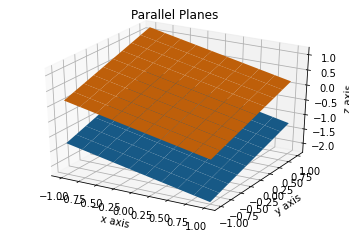
\includegraphics[width=\columnwidth]{solutions/su2021/2/43/c/ASSIGNMENT 5.png}
    \caption{Parallel planes}
    \label{linform/43/c/fig: PARALLEL planes.}
\end{figure}    

    \item 
    We obtain the vertices of the rhombus as follows
\begin{align}
\vec{A} = \myvec{-3\\0},
\vec{B} = \myvec{0\\-3.5},
\vec{C} = \myvec{3\\0},
\vec{D} = \myvec{0\\3.5}
\end{align}
which are plotted in Fig. \ref{quad/45/fig:Rhombus ABCD}.
%
\begin{figure}[ht!]
\centering
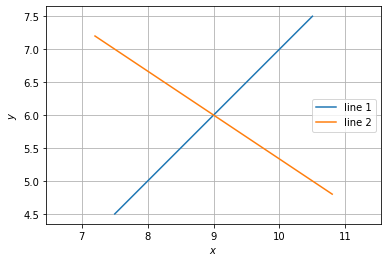
\includegraphics[width=\columnwidth]{solutions/quad/45/figure2.png}
\caption{Rhombus ABCD}
\label{quad/45/fig:Rhombus ABCD}
\end{figure}

    %
\end{enumerate}
\item In the following cases, find the distance of each of the given points from the corresponding plane.
%\newcounter{rowno}
%\setcounter{rowno}{0}
\begin{table}[!h]
\centering
%\begin{tabular}{>{\stepcounter{rowno}\therowno.}cl}
%\multicolumn{1}{r}{No.} & text & abcd\\\hline
% & first  \\
% & second \\
% & third  \\
% & fourth 
%\end{tabular}
\input{./line/tables/3d_ncert.tex}
\caption{}
\label{table:3d}
\end{table}
%
\item 

\item If the coordinates of the points $\bm{A}, \bm{B}, \bm{C}, \bm{D}$ be \myvec{1\\2\\3}, \myvec{4\\5\\7}, \myvec{-4\\3\\-6}, \myvec{2\\9\\2}, then find the angle between the lines $AB$ and $CD$.  
%
\item If the lines 
\begin{align}
\frac{x-1}{-3} = \frac{y-2}{2k} &= \frac{z-3}{2}, 
\\
\frac{x-3}{3k} = \frac{y-1}{1} &= \frac{z-6}{-5} ,
\end{align}
find the value of $k$.
\item Find the  equation of the line passing through \myvec{1\\2\\3} and perpendicular to the plane %
\begin{align}
\myvec{1 & 2 & -5}\vec{x}&=-9
\end{align}
\item Find the shortest distance between the lines 
%
\begin{align}
\vec{x} = \myvec{6 \\ 2 \\ 2} + \lambda_1 \myvec{1 \\ -2 \\ 2}  \text{ and }
\\
\vec{x} = \myvec{-4 \\ 0 \\ -1} + \lambda_2 \myvec{3 \\ -2 \\ -2}  
\end{align}
%
\item Find the coordinates of the point where the line through \myvec{5\\1\\6} and \myvec{3\\4\\1} crosses the YZ-plane.
\item Find the coordinates of the point where the line through \myvec{5\\1\\6} and \myvec{3\\4\\1} crosses the ZX-plane.
\item Find the equation of the plane passing through the point \myvec{-1\\3\\2} and perpendicular to each of the planes 
\begin{align}
\myvec{1 & 2 & 3}\vec{x}&=5
\\
\myvec{3 & 3 & 1}\vec{x}&=0
\end{align}
\item If the points \myvec{1\\1\\p} and \myvec{-3\\0\\1} be equidistant from the plane 
\begin{align}
\myvec{3 & 4 & -12}\vec{x}&=-13,
\end{align}
%
then find the value of $p$.
\item Find the equation of the plane passing through the line of intersection of the planes 
\begin{align}
\myvec{1 & 1 & 1}\vec{x}&=1 \text{ and }
\\
\myvec{2 & 3 & -1}\vec{x}&=-4
\end{align}
%
and parallel to the x-axis.
\item If $\vec{O}$ be the origin and the coordinates of $\vec{P}$ be \myvec{1\\2\\3}, then find the equation of the plane passing through $\vec{P}$ and perpendicular to $OP$.
%
\\
\solution
The normal vector to the plane is 
\begin{align}
\vec{n} &= \myvec{1\\2\\3}
\end{align}
Thus, the equation of the plane is given by
\begin{align}
\vec{n}^T\brak{\vec{x}-\vec{P}} &= 0
\\
\implies \myvec{1 & 2 & 3}{\vec{x}} &= \myvec{1 & 2 & 3}{\myvec{1\\2\\3}}
\\
\implies \myvec{1 & 2 & 3}{\vec{x}} &= 14
\end{align}
%
and is plotted in Fig. \ref{linform/2/55/Plot of the plane}.
\begin{figure}[!ht]
\centering
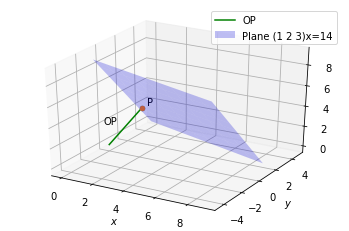
\includegraphics[width=\columnwidth]{solutions/su2021/2/55/PLANE.png}
\caption{Plot of the plane}
\label{linform/2/55/Plot of the plane}
\end{figure}



%
\item Find the equation of the plane which contains the line of intersection of the planes 
%
\begin{align}
\myvec{1 & 2 & 3}\vec{x}&=4 
\\
\myvec{2 & 1 & -1}\vec{x}&=-5
\end{align}
%
and which is perpendicular to the plane 
\begin{align}
\myvec{5 & 3 & -6}\vec{x}&=-8
\end{align}
%
\item Find the vector equation of the line passing through \myvec{1\\2\\3} and parallel to the planes 
%
\begin{align}
\myvec{1 & -1 & 2}\vec{x}&=5
\\
\myvec{3 & 1 & 1}\vec{x}&=6
\end{align}
%
\solution
%The normal vector to the desired plane is perpendicular the normal vectors of both the given planes. Thus
\begin{align}
\vec{n}&=\vec{n_1} \times \vec{n_2}
\\
&=\myvec{1\\-1\\2} \times \myvec{3\\1\\1}\\=\myvec{-3\\5\\4}
\end{align}
and the equation of the line is
\begin{align}
\vec{r}=\myvec{1\\2\\3}+\lambda \myvec{-3\\5\\4}   
\end{align}

\item The planes 
%
\begin{align}
\myvec{2 & -1 & 4}\vec{x}&=5
\\
\myvec{5 & -\frac{5}{2} & 10}\vec{x}&=6
\end{align}
%
are 
%
\begin{enumerate}[itemsep=2pt]
\begin{multicols}{2}
\item Perpendicular
\item Parallel
\item intersect y-axis
\item passes through $\myvec{0\\0\\\frac{5}{4}}$
\end{multicols}
\end{enumerate}
%
\item Find the maximum and minimum values, if any of
the following functions given by 
%
\begin{enumerate}
\item $f(x) = \abs{x+2}-1$
\item $f(x) = -\abs{x+1}+3$
\item $h(x) = x+1, x \in \brak{-1,1}$.
\end{enumerate}
%
\item Using integration find the area of region bounded by the triangle whose vertices are \myvec{1\\ 0}, \myvec{2\\ 2} and \myvec{3\\ 1}.
%
\item  Using integration find the area of region bounded by the triangle whose vertices are (– 1, 0), (1, 3) and (3, 2).
\item  Using integration find the area of the triangular region whose sides have the equations $\myvec{2 & -1 }\vec{x} = -1$, $\myvec{3 & -1 }\vec{x} = -1$ and x = 4.
%
\item Find the area of the region bounded by the line $\myvec{3 & -1}\vec{x} = -2$, the x-axis and the ordinates $x = -1, x = 1$.
\item Find the area bounded by the curve $\abs{x}+\abs{y} = 1$.
\item Using the method of integration find the area of $\triangle ABC$, whose vertices are $\vec{A} = \myvec{ 2\\0 }, \vec{B} = \myvec{ 4\\5 }, \vec{C} = \myvec{ 6\\3 }$.
\item  Using integration find the area of the triangular region whose sides have the equations $\myvec{2 & 1 }\vec{x} = 4$, $\myvec{3 & -2 }\vec{x} = 6$ and  $\myvec{1 & -3 }\vec{x} = -5$.
\item The two equal sides of an isosceles triangle with fixed base $b$ are decreasing at the rate of 3 cm per second. How fast is the area decreasing when the two equal sides are equal to the base ?
\item A tank with rectangular base and rectangular sides, open at the top is to be constructed so that its depth is 2 m and volume is 8 $m^3$
. If building of tank costs
\rupee 70 per sq metres for the base and Rs 45 per square metre for sides. What is the cost of least expensive tank?
\item A point on the hypotenuse of a triangle is at distance a and b from the sides of the triangle.
Show that the minimum length of the hypotenuse is
%
\begin{align}
\brak{a^{\frac{2}{3}}+b^{\frac{2}{3}}}^{\frac{3}{2}}
\end{align}
%
\item Prove that the function $f(x) = 5x – 3$ is continuous at $x = 0, at x = – 3$ and at $x = 5$.
\item Examine the following functions for continuity.
%
\begin{enumerate}
\item $f(x) = x-5$
\item $f(x) = \abs{x-1}$
\end{enumerate}
%
\item Is the function defined by 
%
\begin{align}
f(x)=
\begin{cases}
x, & x \le 1,
\\
5, & x > 1
\end{cases}
\end{align}
%
continuous at $x = 0$? At $x = 1$? At $x = 2$?
\item Find all points of discontinuity of $f$, where $f$ is defined by
%
\begin{enumerate}
\item 
$
\begin{alignedat}[t]{2}
f(x)=
\begin{cases}
2x+3, & x \le 2,
\\
2x-3, & x > 2
\end{cases}
\end{alignedat}
$
%
\item 
$
\begin{alignedat}[t]{2}
f(x)=
\begin{cases}
\abs{x}+3, & x \le -3,
\\
-2x, & -3 < x < 3
\\
6x+2, & x \ge 2
\end{cases}
\end{alignedat}
$
\item 
$
\begin{alignedat}[t]{2}
f(x)=
\begin{cases}
\frac{\abs{x}}{x}, & x \ne 0,
\\
0, & x = 0,
\end{cases}
\end{alignedat}
$
\item 
$
\begin{alignedat}[t]{2}
f(x)=
\begin{cases}
\frac{x}{\abs{x}}, & x < 0,
\\
-1, & x \ge 0,
\end{cases}
\end{alignedat}
$
\end{enumerate}
%
\item Is the function defined by 
%
\begin{align}
f(x)=
\begin{cases}
x+5, & x \le 1,
\\
x-5, & x > 1
\end{cases}
\end{align}
%
a continuous function?
\item Discuss the continuity of the function $f$, where $f$ is defined by 
\begin{enumerate}
\item 
$
\begin{alignedat}[t]{2}
f(x)=
\begin{cases}
3, & 0 \le x \le 1,
\\
4, & 0 < x \le 3,
\\
5, & 3 \le x \le 10,
\end{cases}
\end{alignedat}
$
%
\item 
$
\begin{alignedat}[t]{2}
f(x)=
\begin{cases}
2x, & x < 0,
\\
0, & 0 \le x \le 1
\\
4x, &  x > 1
\end{cases}
\end{alignedat}
$
\item 
$
\begin{alignedat}[t]{2}
f(x)=
\begin{cases}
-2, & x < -1,
\\
2x, & -1 \le x \le  1
\\
2, & x >  1
\end{cases}
\end{alignedat}
$
\end{enumerate}
%
\item Find the relationship between $a$ and $b$ so that the function defined by 	
%
\begin{align}
f(x)=
\begin{cases}
ax+1, & x \le 3,
\\
bx+3, & x > 3
\end{cases}
\end{align}
%
is continuous at $x = 3$
%
\item Prove that the function $f(x) = x$ is continuious at every real number.
\item Is $f(x) = \abs{x}$ a continuous function?
\item Discuss the continuity of the function $f$ defined by 
%
\begin{align}
f(x)  = 
\begin{cases}
x+2 & x \le 1
\\
x-2 & x > 1
\end{cases}
\end{align}

\item Show that the function defined by $g (x) = x – [x]$ is discontinuous at all integral points. Here $[x]$ denotes the greatest integer less than or equal to $x$.
\item For what value of $k$ is the following function 
%
continuous at the given point.
\begin{align}
f(x)=
\begin{cases}
kx+1, & x \le 5,
\\
3x-5, & x > 5,
\end{cases}
\quad x = 5
\end{align}
\item Prove that the function $f$ given by 
\begin{align}
f(x) = \abs{x-1}, x \in \vec{R}
\end{align}
%
is not differentiable at $x = 1$.
\item Prove that the greatest integer function defined by 
\begin{align}
f(x) = \abs{x}, 0 < x < 3
\end{align}
%
is not differentiable at $x = 1$ and $x = 2$.
\item Examine if Rolle's theorem is applicable to the following functions
\begin{enumerate}
\item 
\label{prob:line_eq_rolle}
$
f(x) = \sbrak{x}, x \in \sbrak{5,9}.
$
\item 
$
f(x) = \sbrak{x}, x \in \sbrak{-2,2}.
$
\end{enumerate}
Can you say some thing about the converse of Rolle's theorem from this example?
\item  Examine the applicability of the mean value theorem for all functions in Problem \ref{prob:line_eq_rolle}.
%
\item Find $\lim_{x\to 5} x+10$
\item Find $\lim_{x\to 2} 3x$
\item Find $\lim_{x\to 0}f(x)$ where
%
\begin{align}
f(x)  = 
\begin{cases}
1 & x \le 0
\\
2 & x > 0
\end{cases}
\end{align}
\item Find $\lim_{x\to 0}f(x)$ where
%
\begin{align}
f(x)  = 
\begin{cases}
x-2 & x < 0
\\
0 & x = 0
\\
x+2 & x > 0
\end{cases}
\end{align}
\item Evaluate the following limits
\begin{enumerate}
\item $\lim_{x\to 3}x+3$
\item $\lim_{x\to \pi}\brak{x-\frac{22}{7}}$
\end{enumerate}
%
\item Find $\lim_{x\to 0} f(x)$ where
\begin{align}
f(x) = 
\begin{cases}
\frac{\abs{x}}{x} & x \ne 0
\\
0, & x = 0
\end{cases}
\end{align}
%
\item Find $\lim_{x\to 0} f(x)$ where
\begin{align}
f(x) = 
\begin{cases}
\frac{x}{\abs{x}} & x \ne 0
\\
0, & x = 0
\end{cases}
\end{align}
%
\item Find $\lim_{x\to 5} \abs{x}-5$.
%
\item Suppose
\begin{align}
f(x) = 
\begin{cases}
a+bx & x \ne 1
\\
4, & x = 1
\\
b-ax & x > 1
\end{cases}
\end{align}
%
and if $\lim_{x\to 1}f(x) = f(1)$, what are the possible values of $a$ and $b$?
%
\item If
\begin{align}
f(x) = 
\begin{cases}
\abs{x}+1 & x < 0
\\
0, & x = 0
\\
\abs{x}-1 & x > 0
\end{cases}
\end{align}
%
for what value(s) of $a$ does $\lim_{x\to a}f(x)$ exists?

\item Find the derivative of $x$ at $x = 1$.
\item Find the derivative of $99x$ at $x = 100$.

\item Find the derivative of the following functions:
%
\begin{enumerate}
\item  $-x$
\item  $x+a$
\end{enumerate}
%
\item Integrate the following as limit of sums:
\begin{enumerate}[label = (\roman*)]
\item $\int_{a}^{b}x\, dx$
\item $\int_{0}^{5}\brak{x+1}\, dx$
\item $\int_{-1}^{1}\brak{x+1}\, dx$
\item $\int_{-5}^{5}\abs{x+2}\, dx$
\item $\int_{2}^{8}\abs{x-5}\, dx$
\item $\int_{0}^{4}\abs{x-1}\, dx$
\item $\int_{1}^{4}\sbrak{\abs{x-1}+\abs{x-2}+\abs{x-3}}\, dx$
\end{enumerate}
%
\item Form the differential equation representing the following family of curves 
\begin{align}
\myvec{\frac{1}{a} & \frac{1}{b}}\vec{x} = 1
\end{align}
%
\item Find $\theta$ and $p$ if 
%
\begin{align}
\myvec{\sqrt{3} & 1}\vec{x} = -2
\end{align}
%
is equivalent to
%
\begin{align}
\myvec{\cos\theta & \sin\theta}\vec{x} = p
\end{align}
\item Find the equation of the line which passes through  the point \myvec{-2\\4\\-5} and parallel to the line given by 
\begin{align}
\frac{x+3}{3} = \frac{y-4}{5} = \frac{z+8}{6}. 
\end{align}
\item Find the angle between the following pair of lines
\begin{enumerate}
\item 
\begin{align}
\frac{x-2}{2} = \frac{y-1}{5} &= \frac{z+3}{-3}, 
\\
\frac{x+2}{-1} = \frac{y-4}{8} &= \frac{z-5}{4} 
\end{align}
\item 
\begin{align}
\frac{x}{2} = \frac{y}{2} &= \frac{z}{1}, 
\\
\frac{x-5}{4} = \frac{y-2}{1} &= \frac{z-3}{8} 
\end{align}
\end{enumerate}
\item Find the equation of a plane which is at a distance of 7 units from the origin and normal to \myvec{3\\5\\-6}.
%
\item  For the following planes, find the coordinates of the foot of the perpendicular drawn from the origin
\begin{enumerate}[itemsep=2pt]
\begin{multicols}{2}
\item
$
\myvec{2 & 3 & 4}\vec{x}=12
$
\item
$
\myvec{3 & 4 & -6}\vec{x}=0
$
\item
$
\myvec{1 & 1 & 1}\vec{x}=1
$
\item
$
\myvec{0 & 5 &0}\vec{x}=-8
$
\end{multicols}
\end{enumerate}

%\end{enumerate}
